\usepackage{amsthm}

\newtheorem{theorem}{Theorem}[chapter]
\newtheorem{lemma}           [theorem] {Lemma}   
\newtheorem{folg}           [theorem] {Folgerung}   

\newtheorem{frage}       [theorem] {Frage}   
\newtheorem{question}       [theorem] {Question}   
\newtheorem{aufgabe}       [theorem] {Aufgabe}   
\newtheorem{exercise}       [theorem] {Exercise}  

\newtheorem{proposition}     [theorem] {Proposition}  
\newtheorem{satz}     [theorem] {Satz}  
\newtheorem{fact}{Fact}
\newtheorem{definition}      [theorem] {Definition} 

\theoremstyle{definition} 
\newtheorem{bemerkung}     [theorem] {Bemerkung}  
\newtheorem{beispiel}       [theorem] {Beispiel}  
\newtheorem{example}       [theorem] {Example}  
\newtheorem*{example*} {Example}  
\newtheorem{notation}       [theorem] {Notation}  
\newtheorem*{Faust}[theorem]{Rule of Thumb}
\newtheorem*{Boxx}[theorem]{Concept}

%\section{Exponential Function}

\begin{Definition}{}
 The \emph{exponential function} $\exp:\mathbb{K}\to\mathbb{K}$ is defined as
\[\exp(x)=\sum_{k=0}^\infty\frac{x^k}{k!}.\]
The number
\[e=\exp(1)=\sum_{k=0}^\infty\frac{1}{k!}\]
is called \emph{Euler's number}.
\end{Definition}
For Euler's number holds
\[e\approx 2.718281828459046.\]
We already saw as an example application of the quotient criterion that the above defined series converges for all $x\in\mathbb{K}$. 
Now we present an estimate for $\exp(x)$ if the series is replaced by a finite sum.
\begin{Theorem}{}\label{thm:expest}
 For $n\in\mathbb{N}$ and $x\in\mathbb{K}$ with $|x|\leq1+\frac{n}2$ holds
\[\exp(x)=\sum_{k=0}^n\frac{x^k}{k!}+r_n(x)\qquad\text{with }|r_n(x)|\leq2\frac{|x|^{n+1}}{(n+1)!}.\]
\end{Theorem}
\white{7cm}{
{\em Proof:}
\[
\begin{aligned}
|r_n(x)|&=\left|\sum_{k=n+1}^\infty\frac{x^k}{k!}\right|
\leq\sum_{k=n+1}^\infty\frac{|x|^k}{k!}\\
&=\frac{|x|^{n+1}}{(n+1)!}\cdot\sum_{k=0}^\infty\frac{|x|^{k}}{(n+2)\cdot(n+3)\cdots(n+1+k)}\\
&\leq\frac{|x|^{n+1}}{(n+1)!}\cdot\sum_{k=0}^\infty\frac{|x|^{k}}{(n+2)^k}
=\frac{|x|^{n+1}}{(n+1)!}\cdot\frac1{1-\frac{|x|}{n+2}}
\end{aligned}
\]
Since $|x|\leq\frac{n}2+1=\frac{n+2}2$, we have
\[|r_n(x)|\leq
\frac{|x|^{n+1}}{(n+1)!}\cdot\frac1{1-\frac{1}{2}}=2\frac{|x|^{n+1}}{(n+1)!}
\]
\hfill$\Box$
}

\begin{Theorem}{Properties of the Exponential Function}\label{thm:expprop}
 \begin{enumerate}[(i)]
  \item For all $x,y\in\mathbb{C}$ holds $\exp(x+y)=\exp(x)\exp(y)$.
  \item For all $x\in\mathbb{C}$ holds $\exp(\overline{x})=\overline{\exp(x)}$ ($\overline{y}$ denotes the complex conjugate of $y\in\mathbb{C}$).
  \item For all $x\in\mathbb{C}$ holds $\exp(x)\neq0$ and
\[\exp(-x)=\frac1{\exp(x)}.\]
  \item For $x\in\mathbb{R}$ with $x\geq0$ holds $\exp(x)\geq1$. Where $\exp(x)=1 \Leftrightarrow x=0$.
  \item For $x\in\mathbb{R}$ with $x<0$ holds $0<\exp(x)<1$.
  \item $\exp$ in continuous.
  \item $\exp:\mathbb{R}\to\mathbb{R}$ is strictly monotonically increasing.
  \item $\lim_{x\to\infty}\exp(x)=\infty$ and $\lim_{x\to-\infty}\exp(x)=0$.
  \item $\exp:\mathbb{R}\to(0,\infty)$ is bijective.
  \item For all $x\in\mathbb{C}$ holds $|\exp(x)|=\exp(\Re(x))$.
 \end{enumerate}
\end{Theorem}
{\em Proof:}
 \begin{enumerate}[(i)]
  \item Already shown as an example application of the cauchy product of series.
\item Since we have $\overline{x_1+x_2}=\overline{x_1}+\overline{x_2}$ and $\overline{x_1x_2}=\overline{x_1} \cdot  \overline{x_2}$ for all $x_1,x_2\in\mathbb{C}$, we have
\[\exp(\bar{x})=\sum_{k=0}^\infty\frac{\bar{x}^k}{k!}=\overline{\sum_{k=0}^\infty\frac{{x}^k}{k!}}=\overline{\exp(x)}.\]
\item By definition of $\exp$, we have $\exp(0)=1$. From (i), we get $\exp(x)\cdot\exp(-x)=\exp(x-x)=\exp(0)=1$. Then the statement follows.
\item From $x\geq0$, we get
\[\exp(x)=\sum_{k=0}^\infty\frac{x^k}{k!}=1+\sum_{k=1}^\infty\frac{x^k}{k!}\geq1.\]
It is immediately clear that equality only holds for $x=0$.
\item If $x<0$, we get from (iii) that $\exp(-x)>1$. Then, $\exp(x)=\frac1{\exp(-x)}<1$.
\item First we show that $\exp$ is continuous at $0$.
\white{11cm}{
Let $(x_n)_{n\in\mathbb{N}}$ be a~sequence converging to $0$. By Theorem~\ref{thm:expest} holds for (small enough) $x_n$ that
$|\exp(x_n)-1|=|r_0(x_{n})|$ with
\[|r_0(x_n)|\leq2\frac{|x_n|}{1!}=2|x_n|.\]
Therefore,
\[\lim_{n\to\infty}|\exp(x_n)-\exp(0)|=\lim_{n\to\infty}|\exp(x_n)-1|=\lim_{n\to\infty}|r_0(x_{n})|=0\]
which proves the continuity at $0$. In order to show continuity on the whole real axis, we assume that $(x_n)_{n\in\mathbb{N}}$ converges to $x_0\in\mathbb{R}$ and make use of
\[\lim_{n\to\infty}\exp(x_n)=\exp(x_0)\lim_{n\to\infty}\exp(x_n-x_0).\]
Since $(x_n-x_0)_{n\in\mathbb{N}}$ converges to 0, the above limit on the right hand side converges to 1 (due to the continuity in 0). Therefore, we have
\[\lim_{n\to\infty}\exp(x_n)=\exp(x_0)\]
which proves continuity of $\exp$ at $x_0$.
}
\item Let $x_1,x_2\in\mathbb{R}$ with $x_1> x_2$. Then we have $x_1-x_2>0$ and thus, by (iv), $\exp(x_1-x_2)>1$. Since $\exp(x_2)>0$, we have
\[\exp(x_1)=\exp(x_2)\exp(x_1-x_2)>\exp(x_2).\]
\item The fact $\lim_{x\to\infty}\exp(x)=\infty$ follows, since we have for $x>0$ that
\[\exp(x)=\sum_{k=0}^\infty\frac{x^k}{k!}=1+x+\sum_{k=2}^\infty\frac{x^k}{k!}>1+x.\]
The statement (iii) then directly implies $\lim_{x\to-\infty}\exp(x)=0$.
\item The injectivity of $\exp:\mathbb{R}\to(0,\infty)$ follows from (vii). It remains to show surjectivity. Let $y\in(0,\infty)$.\\
Since $\lim_{x\to-\infty}\exp(x)=0$, there exists some $x_0\in\mathbb{R}$ such that $\exp(x_0)<y$.\\
Since $\lim_{x\to\infty}\exp(x)=\infty$, there exists some $x_1\in\mathbb{R}$ such that $\exp(x_1)>y$.\\
Now, by the Mean Value Theorem, (remember that $\exp$ is continuous), there exists some $x\in\mathbb{R}$ with $\exp(x)=y$.
\item Let $x=x_1+ix_2$ with $x_1=\Re(x)$, $x_2=\Im(x)$. Then
\[
 | \exp(x) | =
|\exp(x_1+ix_2)|=|\exp(x_1)\exp(ix_2)|=|\exp(x_1)||\exp(ix_2)|.\]
If we now show that $|\exp(ix_2)|=1$, the result is proven:
Making use of (ii), we obtain
\[|\exp(ix_2)|^2=\exp(ix_2)\cdot\overline{\exp(ix_2)}=\exp(ix_2-ix_2)=\exp(0)=1.\]\hfill$\Box$
\end{enumerate}

%  \begin{figure}[h!]
%  \begin{center}
%  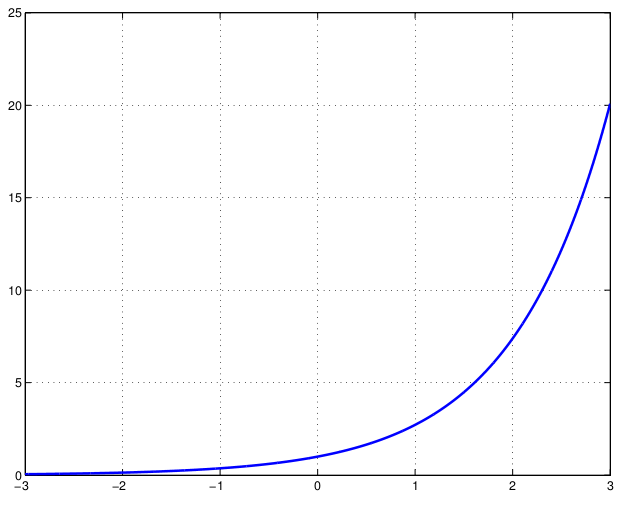
\includegraphics[width=0.81\textwidth,angle=0]{pics/exp.eps}
%  \caption{Graph of the exponential function}\label{fig:exp}
%  \end{center}
%  \end{figure}

